\chapter{Collaborative tools}
\newcommand{\moodle}{\textsf{Moodle}}
\newcommand{\Moodle}{\textsf{Moodle}}

\notesurl{desktop2}

\begin{note}
  This is the fifth, two hour, lab.

  There was a feeling that the getting started with Moodle material might be a little light for a 2 hour session, so perhaps put some more Desktop oriented material in here as well.

  Has change of position (?) of this lab made any difference to how we tell students about first tutorial?

  Do we need some breakout boxes in this script?
  
  
  which supports COMP10120. You should also use this lab session to complete the \emph{Individual Learning Profile} questionnaire which is hosted inside \moodle.

\moodle\ is a \emph{Virtual Learning Environment} (VLE) that allows the classroom to extend onto the web.
  
\end{note}


\section{Getting started with \moodle}
\label{sec:introduction-moodle}

In this lab session you'll be introduced to the \moodle\ Virtual Learning Environment (VLE). \moodle\ is an Open Source platform designed to support face-to-face teaching by providing an online place to upload resources for course units. It also provides useful  tools such as discussion forums and quizzes. We use \moodle\ for several of our course units, which typically have a single `course unit site' within our \moodle\ environment.

%Why is Moodle being used for COMP10120
\moodle\ has several features which make it well suited to supporting this course-unit. These include:
\begin{itemize}
\item It's one useful way of communicating with your tutor and members of your tutor group 
\item It allows us to give each group a wiki which you'll use to collaboratively document your project work.
\item It provides a structure to help organise activities you should be doing on a week-by-week basis.
\end{itemize}

Log in to \moodle\ by pointing your web browser at: \urlnop{moodle.cs.man.ac.uk} and using your University credentials. 

After successfully logging into \moodle\ for the first time, you'll be presented with a form to complete the details of your \moodle\ profile. Add your first and last names; your email address; the city/town where you live (for most people this will be Manchester); and add a short description of yourself. Select the `Update profile' button to complete your \moodle\ registration. Assuming that worked okay, the next page to appear will be the \moodle\ home page (see  Figure~\ref{figure:moodle-home})

\begin{figure}
\centerline{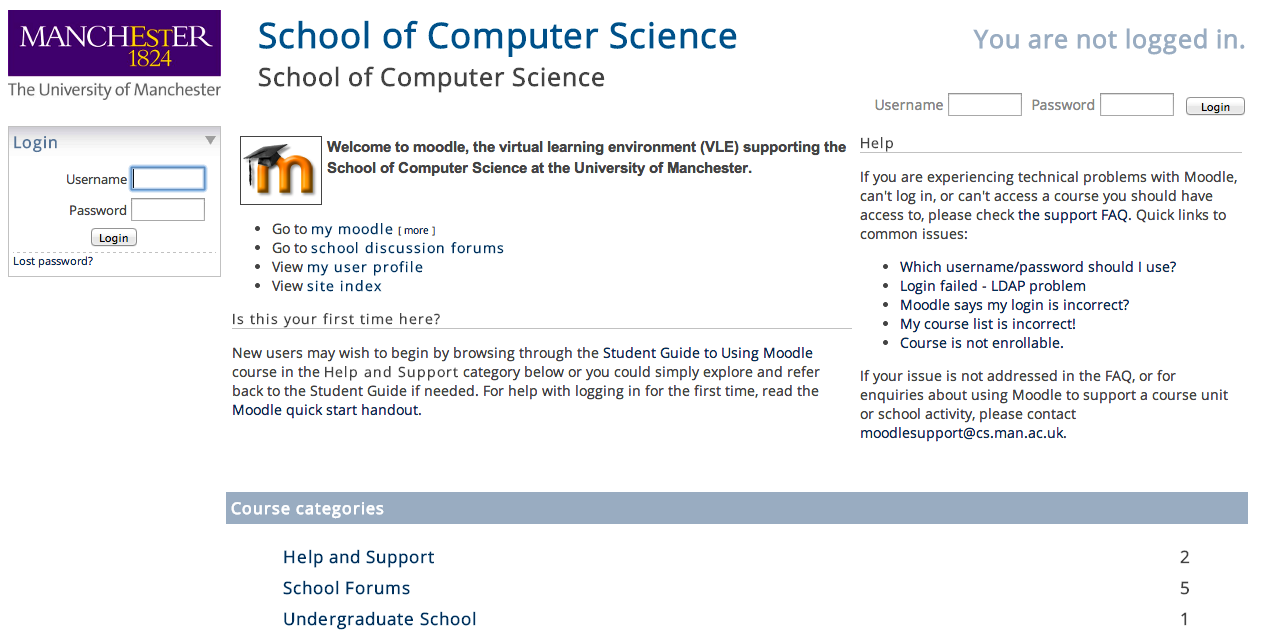
\includegraphics[width=15cm]{images/moodle-home}}
\caption{Moodle Home Page}\label{figure:moodle-home}
\end{figure}

Take a few minutes to browse though the \emph{Getting started with \Moodle} guide which is deliberately located outside the \moodle\ environment so that you can get at it in case you're having problems with \moodle\ itself. You can find it at: \urlnop{octette.cs.man.ac.uk/moodleintro} (see Figure~\ref{figure:moodle-start}).

\begin{figure}
\centerline{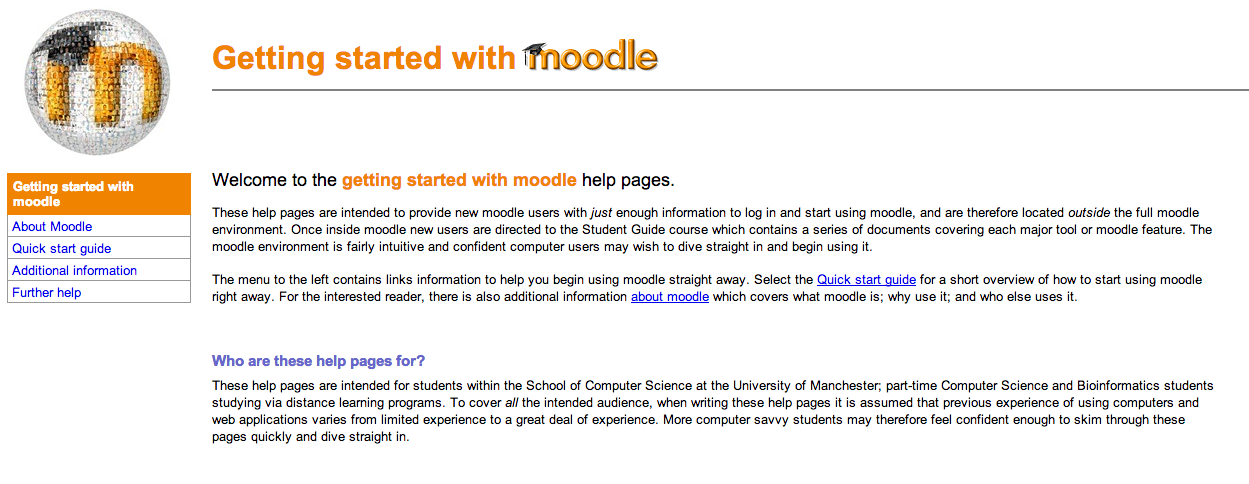
\includegraphics[width=15cm]{images/start-moodle-page}}
\caption{Getting started with Moodle}\label{figure:moodle-start}
\end{figure}

\subsubsection*{Brief overview of the \moodle\ home page}
\label{sec:brief-overv-moodle}


The \moodle\ home page lists several categories in which \moodle\ course unit sites are organised (make sure you scroll down to see them all). \moodle\ course unit sites exist for many, but not all, course units within your degree programme. There are also a number of \moodle\ sites that provide support to staff and students in other ways, such as a general CS help sites and the Staff Student Consultative Committee public site.

You can find links to sites by either locating the link in the appropriate category, for example look in \emph{Undergraduate School/First Year} for COMP10120; or you can enter \emph{COMP10120} into the \emph{Search courses} field at the bottom of the course list and select the course unit title from the search result(s).

Other things to look out for on the front page include the link to your \moodle\ user profile and the link to the \emph{my moodle} feature. We'll come back to these later on.


%Your turn


Make sure you can find the COMP10120 course unit site and are able to access it. To get back to the \emph{\moodle\ home page} you should click on the \moodle\ link in the navigation bar underneath the course unit title at the top of the page. This is always the first element in the link trail. If you navigate further into the course unit site, to return to the \emph{course unit site front page} just click on the COMP10120 link in the navigation bar. This is always the second element in the link trail.

Now locate the course titled \emph{Student Guide to Using Moodle} (in the category \emph{Help and Support}). Have a browse through what help material is provided here. You may wish to revisit this site to learn how to use one of the \moodle\ activities or understand one of \Moodle's features.

\subsection{The COMP10120 course unit site}
\label{sec:comp10120-course-uni}


If you haven't already, navigate to the COMP10120 site and start to look at how the site is structured and what tools have been provided (see Figure~\ref{figure:101-moodle-page}).
Things you should note about the structure of the site:

\begin{figure}
\centerline{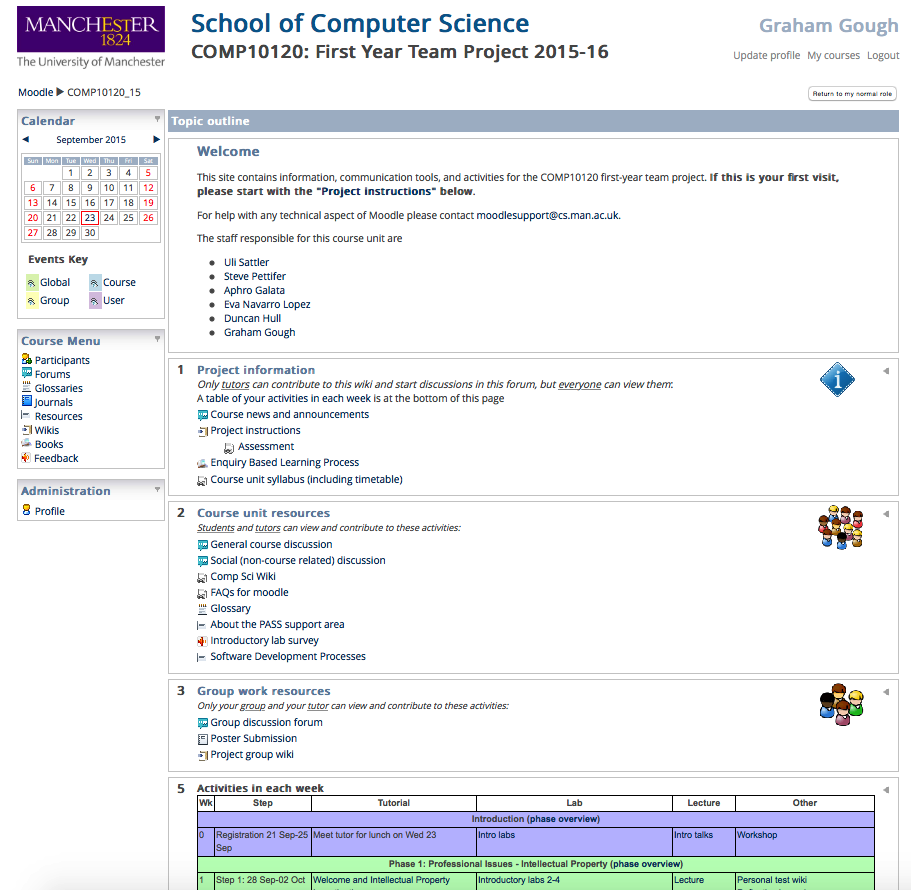
\includegraphics[width=15cm]{images/101-moodle-page}}
\caption{COMP10120 Moodle Home Page}\label{figure:101-moodle-page}
\end{figure}


\begin{itemize}
\item 
All instructions for the course unit are located in the \emph{Project information} area towards the top of the site. Take a look at each of the links in this area. In particular, familiarise yourself with the front page of the \emph{Project instructions} and read at least the \emph{Introduction to the tasks and activities} (and then click through to the \emph{Phases and Tutorials} page to get an idea of the course unit structure).

\item Back on the course unit site, the next section is called \emph{Course unit resources}. If you have a query about the course unit, please use link to the \emph{General Course Discussion Forum}.

\item The next section is called \emph{Group work resources}. This is your tutor group's area and should be used to communicate with members of your team (by using the forum) and to document your work (in the wiki).

\item Finally, the bottom of the course unit site has a table of all your activities for this course-unit. The different phases are colour-coded to help you spot the one you want. The row for each week contains links to information about what you should be doing in that week and tools/resources applicable to the week. (Don't forget to read the \emph{phase overview} first.)

  The \emph{Other}  column includes resources for your personal use, that you are expected to complete over the course of the year. In particular you should note the \emph{reflective journals} for each week of the first semester. You are expected to reflect on the questions detailed inside the journal each week.
\end{itemize}

% The remaining instructions for this lab session can be found
% directly within \moodle\ itself. Click on \emph{Introduction to \Moodle} % in the \emph{Lab} column for \emph{Step 1} in the green (\emph{Phase 1}  section.

\subsection{Lab deliverables}
\label{sec:lab-deliverables}

\begin{note}
  Do we want a list of deliverables for each lab? Should they be at the start of the script?
\end{note}

By the end of this lab session, ensure you have completed the following tasks.

\begin{itemize}
\item 
Posted a welcoming message to your tutor group (see Using forums below).

\item Create your set of practise wiki pages (see Using wikis below).

\item Completed the Individual Learning Profile questionnaire
\end{itemize}

There are also a number of optional tasks you should aim to complete if you have time during the lab.

\subsection{Using forums}
\label{sec:using-forums}


Most of you will have used discussion forums in some way or another, whether on your favourite social networking site or on some other website. \Moodle's forums aren't too different to any other, however, you should note a few things:

Most forums are configured so that copies of each posting will be emailed to other course unit members. In a group forum, copies are only emailed to other group members; in a course forum copies are emailed to everyone.

In most cases you will have the option to remove your subscription to such emails. Please don't do this, at least not at the moment.

In your user profile you have the option to receive \moodle\ emails as a single daily digest rather than as multiple emails each day; if you're finding you're getting a lot of email from \moodle\ this might be a sensible option to select (but keep it mind that you'll lose some of the immediacy of receiving individual emails). 

You might not be able to post messages in all forums. Some forums (e.g. course announcement forums) will only allow tutors to start new topics of discussion, but will allow students to reply to those topics once started.

%Your turn
Visit your Group discussion forum on the COMP10120 site and click on \emph{Add a new discussion topic}  to begin a new discussion thread. Write a short forum posting to introduce you to your other group members and your tutor. Let them know where you are from, tell them a little bit about yourself. Warning: the current in-line HTML in \moodle\ can sometimes misbehave, especially if you try to apply lots of formatting. Therefore concentrate on content rather than presentation.

Note that your discussion posting won't be emailed to the other members of your group until about 30 minutes after you submit the posting. This is to allow time for you to edit it in case you spot a mistake.

If you want to find out more about using discussion forums, look through the \emph{How to use the forums}  help book in the \emph{Student Guide to Using \Moodle} course. There is also a help book called \emph{Using \moodle's HTML editor} which you may also find useful.

\subsection{Using wikis}
\label{sec:using-wikis}


You have almost certainly come across wikis before, and will no doubt have looked things up in \wikipedia{Wikipedia}{Wikipedia}, the world's biggest wiki, many times. Unlike many other online collaboration systems which constrain users in various ways by pre-determining the type of content that can be create (for example sites like Instagram and Flickr are designed for sharing photographs, where as Soundcloud is for sharing audio), and also categorising users as having different types of access (e.g. administrators, moderators, regular users and so forth), the technology behind wikis typically takes a very liberal approach to both users and content. They generally allow any user to make any kind of change to any kind of content, and rely on \textit{social} conventions established by the community to keep things sane. In particular, every edit, deletion and addition to the wiki is stored, providing a complete history of wiki changes. Old versions of pages and be retrieved and compared to new versions of pages. Wikis are typically edited using a simple mark-up syntax where the focus is on content rather than fancy presentation.


As well as creating sites like Wikipedia, wikis are frequently used by software development teams to document their project. The ability to look back to previous versions of documents and the for multiple authors to collaborate on producing the documentation without having to worry too much about `process' is particularly useful in such environments.

During COMP10120 you'll required to document many aspects of your work using a group wiki provided by \Moodle. \Moodle's wiki isn't as powerful as others you may have come across as it is primarily tailored towards teaching, but it does allow you to use \Moodle's standard in-line HTML editor to help you with formatting.

%Your turn
In the bottom \emph{Resources for individual use} section of the COMP10120 site you will find a link to a wiki called \emph{Personal test wiki} which is private for you and you only. It is provided to allow you to practise how to use \moodle\ wiki syntax before you start using your shared group wiki. If you have used a wiki before then you may find \Moodle's wiki syntax is slightly different to that which you are used to.

For this short exercise you will need to read through some of the help documentation hosted inside \moodle. In a new window or tab navigate to \urlnop{moodle.cs.man.ac.uk} again and enter the \emph{ \emph{Welcome to the Student Guide to Using \Moodle} }course in the \moodle\ \emph{Help and Support}  category (you may be asked to 'enrol' on this course, just select 'Yes'). Scroll down to the section about Wikis and select the \emph{How to use the wiki tool} book.

The aim of this short exercise is to create a simple wiki page with two or three wiki links to other pages; incorporate an image; and attach and link to a binary (non-image) file. It is important that you follow this mini-tutorial through to the end as it will ensure you know how to do all the basic tasks needed to help build your own group wiki during the project.

For the purposes of this mini-tutorial you are asked to create a small wiki about yourself.

Start by opening your Personal test wiki. You will be presented with the \moodle\ editor which won't contain any content yet. Enter a title for the page, something like \emph{About Me} will do.

Select the \emph{Save} button. You should now see the first page of your wiki with the content you just added. Now select the \emph{Edit} tab so that you can add more content.

Create a short bullet list containing the items \emph{My hobbies},  \emph{My music}  and \emph{My files}  Save the page again and check the results, then select the Edit tab again. Now turn the three items into wiki links. To do this, just put a single set of square brackets around each of the terms, like this: \emph{[My hobbies]}  \emph{[My music]}  \emph{[My files]}  Save the page again and look at what just happened. If everything worked correctly each term enclosed in square brackets should now look like this: term? (emboldened text followed by a hyperlinked question mark).

Select the question mark symbol on the \emph{My hobbies} term. Note this opens up a new wiki page called \emph{My hobbies} for you to populate with content. Add some text to describe a few things about what you like to do with your time and then select Save.

This is the basic process by which you build up a wiki into a series of linked pages. Note that at the bottom of the page you just created is a list of \emph{Referring links}  This means \emph{a list of pages that link to this one}  Select the link back to the front page.

In the Student Guide to Using \moodle\ course look at the help book on wikis and read the chapter titled \emph{Unique names for pages}  in particular instructions on how to make the link text different from the linked page name. Now go back and change your first wiki page so that the link to the page \emph{My hobbies} contains the link text \emph{My interests} (but still points to My hobbies). Your list should now contain the items \emph{My interests},  \emph{My music}  and \emph{My files} 

Now go back and select the question mark link for the \emph{My music} link and add some content to this page too. You could write about music you love (or music you hate!).

In the last part of this mini-tutorial, you will need to add a small picture to your wiki and a small file. First we need some files to play with. If you have a small picture that you took yourself, great, you own the copyright on it. Create a small text file using any text editor containing any text you like. If you don't have a picture to use and can not source a copyright free image, you will find a link to an example image in the summary text box of the wiki above the first page. There is also a link to a sample text file there too.

In the Student Guide to Using \moodle\ course look at the help book on wikis and read the chapters titled \emph{Attaching binary files} and \emph{Linking to attached files}  From your wiki's front page select the question mark link for the \emph{My files} link to create its page content. Attach your text file to the page from the wiki's Attachments tab as described in the \emph{Attaching binary files} chapter of the help book. Then return to the edit tab and add the following text:

\emph{Wikis allow users to attach files, such as this one here}  

Turn the word \emph{here} into a link to the text file you just uploaded following the instructions in the \emph{Linking to attached files} chapter of the help book.

Carefully read the chapter of the help book titled \emph{Incorporating images}  Now add the following text and add the image you grabbed earlier below the text.

\emph{Wikis also allow users to incorporate images such as this one.} 

Experiment with changing the alignment of the image as described in the help book.

Finally, browse through the remaining documentation in the Wiki help book so that you have an overview of what other information is there and can refer back to it in the future if needed. If you have any questions about how to use the wiki tool, post a message to the General course unit discussion forum.

\subsection{Individual Learning Profile questionnaire}
\label{sec:indiv-learn-prof}

Before the end of the lab session make sure you complete the \emph{Individual Learning Profile questionnaire}. You will find it in the \emph{Resources for your individual use} section at the bottom of the \moodle\ course unit site. This activity is to help you to reflect so that you can understand your own basic skills and abilities required for your academic life. It may also be looked at by your personal tutor so the School can be better placed to address your particular needs during your time in the School of Computer Science. This information will only be visible to you, to your tutor and to the course unit organisers.

\subsubsection*{Writing your journal}
\label{sec:writing-your-journal}


One of the aims of this course unit is to encourage you to develop the habit of thinking about the way you are learning and working, and trying to identify ways in which these could be improved. The process of reflection is key to this, but is not something that comes naturally to many of us. In most week slots of the course unit site you will find an instance of the Journal activity. The summary text of each journal contains prompts to aid your reflection that week. The journal is very simple \moodle\ tool which provides you with an editable text area supported by \moodle\ HTML editor. Selecting the \emph{Start or edit my journal entry} button opens your journal. Any entries you put into your journal will be completely private to you and your personal course unit tutor. A limited number of the course unit organisers have access to all students journals, but will respect your privacy and will not be looking at them.

At some time towards the end of this week, start your journal entry for the current week and post your answers the prompts provided.

\subsection{What else is on \moodle?}
\label{sec:what-else-moodle}


As well as course unit sites for many of your course units, there are also a number of open areas within \moodle. Within the \emph{Support Forums} category you will find a number of sites where you can seek help about specific areas within computer science, e.g. the C / C++? Programmer's Forum. The \emph{Student / Staff Groups} category includes a site where you can post up questions or topics of discussion for the Staff Student Consultative Committee. All these open courses are indicated by the guest user icon (a small person icon or a side-on face depending on your chosen \moodle\ theme). Have an explore and see what is there. More open site are likely to be added over the year.

\subsection*{Playing and personalising}
\label{sec:play-pers}


If you have time left in the lab session, spend some time personalising your \moodle\ account. Things you could do include:

Uploading a small photo or image to represent yourself to your \moodle\ profile.

%Personalising your my \moodle\ area.

Take a closer look at the advanced options in your \moodle\ profile and investigate what they do (read up about this in the \moodle\ help course books first).


 Look ahead on the COMP10120 site to get a feel for what you will be doing over the coming year.



\section{Git and GitLab}

During your time at school or college, you'll no doubt have written essays and assignments that took more than one session to complete, and you've probably experienced some annoyances associated with transferring the files containing your work between different machines. Perhaps you started writing on a PC at college, took it home to work on a bit more, and finished it off in a library or on a laptop in a cafe. You may have moved the file around using a cloud-based system like Dropbox or Google Drive, or perhaps you transported it around with you on a USB drive. In any case, it's more than likely that at some point you'll have got yourself muddled up working out which version of the file is the latest, or needed to undo some changes and had to remember which version of the file to go back to. If you've been unlucky, you may have lost important changes along the way, or got to a stage where it feels impossible to undo some unwanted change that you've made because it affects so many different parts of your work that you don't know how to remove their effect without messing up your whole document. If you've ever tried to work collaboratively on a project with someone else, you'll probably have found it quite hard to co-ordinate changes so that things you do don't trample on things that someone else is working on at the same time. 

These are all well-known problems associated with doing any kind of writing or project work that takes more than a few minutes to complete, where you're using multiple machines and/or are working with other people; and as you work on more complex projects over longer periods of time and with bigger groups, the bad news is that these problems all get worse. You can, to a certain extent improve the situation by sticking to certain conventions, such as making regular backups of your work with particular kinds of filenames, or promising always to email your collaborators before you make a change to anything and emailing them again when you've finished your changes. But these informal `social agreements' easily collapse when you are tired or stressed, leaving you with a mess to clear up. The good news is that there are industry-standard ways of dealing with these problems, and in the last part of today's session we're going to introduce you to the basics of version control using Git and Gitlab. 

Git and gitlab are tools to help you manage change. Whether you're working on something on your own or as part of a team, a little effort spent learning how to use these tools now will save you significant amounts of pain and hassle later on. 

Git is a version control system, and is one of the most popular of the thirty or so different systems in use today. It is arguably one of the most powerful and flexible version control systems available, and this does mean that your first contact with it can be a little daunting; but if you follow our instructions carefully and don't get too hung up on the bits that we're having to skim over to keep things simple, you'll soon get the hang of things. 

GitLab is a web-based interface to git which makes it easy (at least, easier) to set up projects and teams for collaborative work. Mastering any version control system takes a long time, and you may find in the early days that using git feels as though its more hassle than its worth --- but version control is a crucial skill for any modern computer scientist, and its important that you get used to the principles right from the start of your degree. And trust us, at some point it is going to save you an enormous amount of trouble!

In combination git and gitlab provide mechanisms for:
\begin{itemize}
\item safely moving files from one machine to another without losing changes in the process. You'll probably find this useful early on, and essential when you start working on your group project,
\item tracking changes that you've made so that you can safely undo things that you later decide you don't want, and
\item keeping things under control when you're working with others on a shared piece of work.
\end{itemize}

Today we're going to keep things as simple as possible, and are just going to use git and gitlab for the first of these things; moving files between machines. 

Before we can start to use the tools properly, there's some housekeeping that we need to do. 

\subsection{Configuring git}

Git has already been installed on the school's system, but you'll need to set up some things that are specific to your user before it will work sensibly. 

Fire up a terminal, and enter the following commands:

\begin{ttoutenv}
git config --global user.name "[YOUR NAME GOES HERE]"
git config --global user.email "[YOUR UNIVERSITY EMAIL GOES HERE]" 
\end{ttoutenv}

Hopefully the purpose of these commands is self-explanatory; you're just telling git who you are and how to contact you by email if it needs to. The next bit of configuration is a bit more mysterious, and explaining what it does would require more explanation than is sensible here, so for now just treat these next instruction as a thing you have to do:

\begin{ttoutenv}
git config --global push.default simple
git config --global branch.autosetuprebase always 
\end{ttoutenv}

The next few instructions are optional, but make the output of git nicer to read, so we recommend you also do:

\begin{ttoutenv}
git config --global color.ui true
git config --global color.status auto
git config --global color.branch auto 
\end{ttoutenv}

and finally you should configure git to use whatever editor you've decided is your favourite at the moment, for example:

\begin{ttoutenv}
git config --global core.editor nano 
\end{ttoutenv}

Check that you've typed these correctly by using the command \ttout{git config --list}. You should see all the things you've entered just now, along with a few other bits of default configuration that were set automatically for you by the system (you can safely ignore these for now).


\subsection{Setting up gitlab}

Next we're going to set up gitlab. Point your browser at the School's installation of gitlab at:
\\
\url{http://gitlab.cs.man.ac.uk}
\\
and log in with your University credentials. You should see Gitlab's `dashboard' page and not much else (see Figure \ref{figure:gitlab-first-login}). Go to the `My Profile' section of gitlab using the icon at the top right of the page, and fill in any details about you that you're comfortable sharing with other students and staff within the school. At a minimum you should make sure that your Name and Email are set correctly; the other fields are optional (if you'd like your gitlab account to have an avatar image, you'll need to sign up for a Gravatar account, which is a bit of a nuisance but not that hard). 

\begin{figure}
\centerline{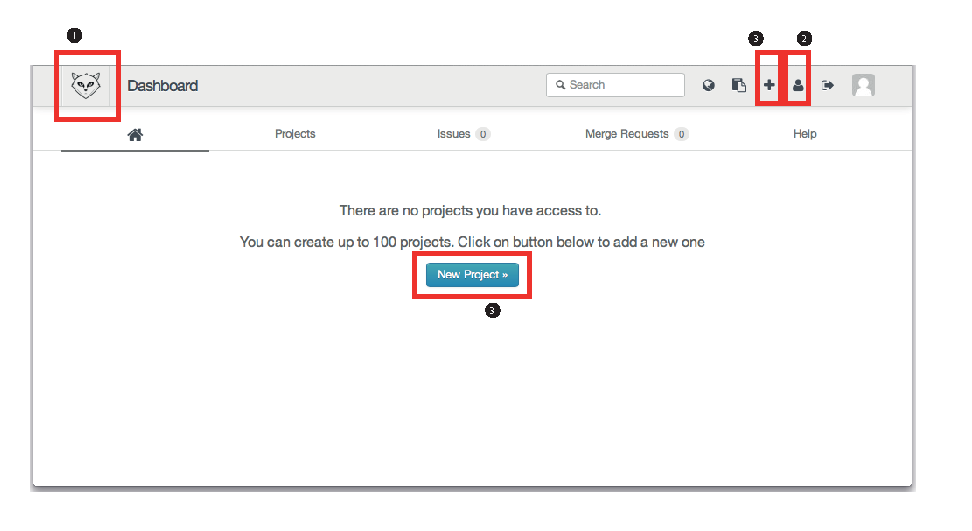
\includegraphics[width=15cm]{images/gitlab-first-login}}
\caption{First login to Gitlab. \protect\circled{1} The Gitlab logo (a sort of raccoon thing) will bring you back to the dashboard; useful if you get lost in gitlab's structure; \protect\circled{2} the user-profile allows you to add more information about yourself, and optionally connect up to Gravatar to give you a user icon; and \protect\circled{3} various ways to create a new project.}\label{figure:gitlab-first-login}
\end{figure}

Select thew `New Project' button from the icons at the top right. Enter \ttout{aboutme} as the project name, and hit `Create project'. You'll see a page similar to Figure \ref{figure:gitlab-new-project}. Notice that the `Git global setup' section contains the commands that you used in the previous section to set up your git configuration; so you don't need to do that again. There are also two other sections of code on how to `create repository' or use `Existing Git Repo?'. Ignore both of these for now and instead follow the instructions here (notice at the top of the gitlab page a warning that `You won't be able to pull or push project code via SSH until you add an SSH key to your profile' -- we need to fix that first). Click on the `add an SSH key' link (marked with \protect\circled{1} on Figure \ref{figure:gitlab-new-project}), which will take you to the SSH key upload page which looks something like Figure \ref{figure:gitlab-ssh}.

\begin{figure}
\centerline{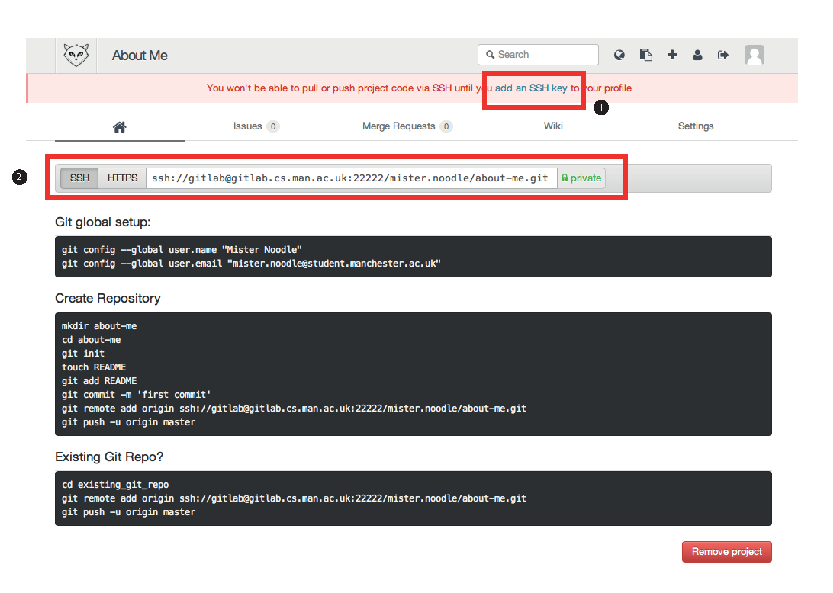
\includegraphics[width=15cm]{images/gitlab-new-project}}
\caption{Creating a new project in Gitlab. \protect\circled{1} You will need to use the  `add an SSH key' link to upload your public key before you can communicate between git and gitlab, and the URL given in \protect\circled{2} can be used from the command line to clone and push this project.}\label{figure:gitlab-new-project}
\end{figure}

\begin{figure}
\centerline{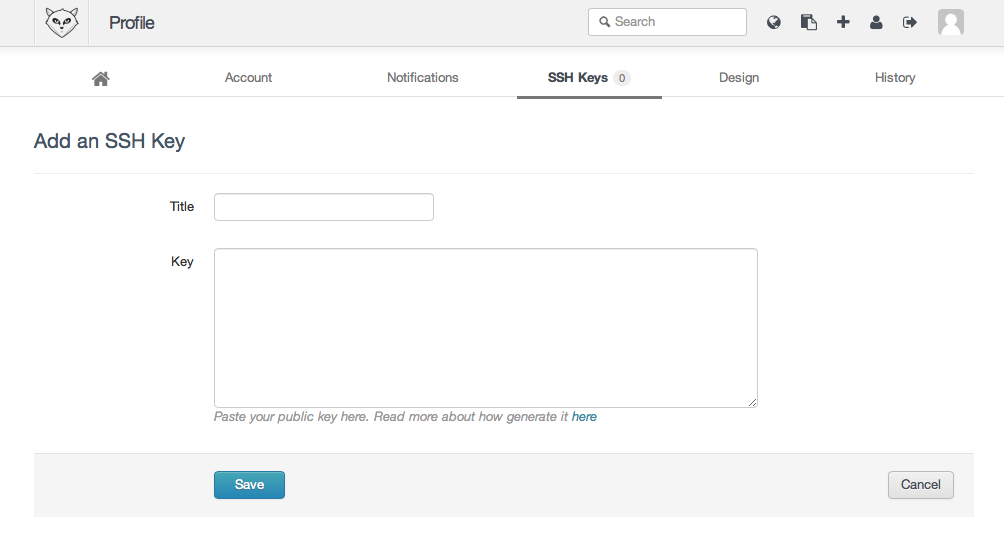
\includegraphics[width=13cm]{images/gitlab-ssh}}
\caption{Adding a SSH key to Gitlab. Once you have used \ttout{ssh-keygen} to create the key, paste the text into the `Key' box; if your key is valid then the title will be filled in for you.}\label{figure:gitlab-ssh}
\end{figure}


You'll now need to set up a means of securely identifying yourself to Gitlab from whichever machine you're using at the time; this is done by creating what's called a `ssh key'. In a terminal, type

\begin{ttoutenv}
ssh-keygen -t rsa -C "[YOUR UNIVERSITY EMAIL]"
\end{ttoutenv}

to create yourself a SSH key. When prompted `Enter file in which to save the key' just press return to accept the default, and the same for `Enter passphrase' twice.  For now don't worry too much about exactly what a SSH key is -- we'll just treat it as a way of identifying yourself to the Gitlab server. 

Look in a directory called \ttout{~/.ssh} and you'll find two new files have been created called \ttout{id\_rsa} and \ttout{id\_rsa.pub}. The first of these is the \textit{private} part of the SSH key that's just been generated for you, and you should keep this secret. The second of these is the \textit{public} part of the key, and this is the bit you need to hand over to gitlab for it to be able to identify you. Use the command

\begin{ttoutenv}
$ less ~/.ssh/id_rsa.pub
\end{ttoutenv}
% $
to display the contents of your public key. You should see something like:

\begin{ttoutenv}
  
  ssh-rsa  AAAAB3NzaC1yc2EAAAADAQABAAABAQDTfAF0KxG94oUJLUER5Ci5HaoEtdi8KI0S+
  iro3EvVkQebW2V3nCaCLAHLmgmINm/NFW5bvbUq7bu2CxFlVBEQqa1idZBLceXKRi1SFtG+
  EzFENyzZBsIDU0IhfQX4qyxgqe0A3ortyAwm2/+0neu74RT0YK3gQI+wyxsFFoCzbahiDJisK
  /vKmqvwowb/Rrl3OZpX9ZO3QA9lgILLVy3J4VpAhR+05MyuM/Bzh/pYk5NIQivedUEduIJXLOetj/
  UnxlH9WbEPEIiDPvzrkb3xI98rLRSlh2hH89nc1SUfVEhY62RQWN7sbXPu+fFck7Dom9wE/
  YAG66Dbl30OsmFh mister.noodle@manchester.ac.uk

\end{ttoutenv}


which starts with \ttout{ssh-rsa}, ends with your email address, and has a load of apparently random characters in between. Select this text (making sure you don't accidentally select any extra newlines or spaces either side of it) and 
Copy and Paste the whole of the SSH key into the `Key' box on the gitlab page. If you've done this correctly, gitlab will spot the email from your key and use this as the `Title' field, in which case just press the Save button. Gitlab will complain if it's not a valid key or has extra spaces or newlines at this point; if you're stuck here grab a demonstrator to help you. 

Once you've uploaded your public key to gitlab, you're ready to put your first bit of content into the `aboutme' project that you've just created. 

Click on the gitlab logo at the top left of the gitlab page to get back to the dashboard, and select the `aboutme' project that you created a moment ago.  Back at your terminal command prompt change to the directory called `aboutme' that you copied over from the Pi at the end of the last session; this should contain at least three files if everything has gone to plan: a bit of HTML about you, a photograph of your, and whatever image you drew using Inkscape (if for whatever reason you didn't get as far as that part in the last session, there's a default set of files you can use; copy them from \ttout{/opt/info/courses/COMP101/aboutme} into a directory called \ttout{aboutme} in your home directory and press on.)

\begin{note}
 Need to set this up in /opt/info
\end{note}

In your \ttout{aboutme} directory, type the following command:

\begin{ttoutenv}
$ git init
\end{ttoutenv}

which tells git that you're about to put this directory under its control; this is known as initialising a repository. Git will respond by telling you that it has `Initialized empty Git repository in ' followed by the full pathname of your \fname{aboutme} directory. 

Type
\begin{ttoutenv}
$ git status
\end{ttoutenv}

and you'll see a message from git that, amongst other things tells you that there are `untracked files' (these should appear in red). 

Now we need to tell git which files we want it to track for us. For each of the three files in that directory run a command along the lines of 

\begin{ttoutenv}
$ git add [FILENAME]
\end{ttoutenv}

% $

replacing [FILENAME] with each of the three file names in turn. Once you've done this, run \ttout{git status} again,, and this time you should see that there are a list of `Change to be committed' and all the files that you'd just added should appear in green. 

Now git knows which of the files in this directory you want to track (which in this case is all of them), we want to do our first `commit', which tells git that we've made a set of changes that we want to keep together: in this case the `changes' are to create the files in the first place; later one we'll go through a similar pattern of \ttout{git add} and {git commit} whenever we've done a set of changes that we think we are happy with. 

The \ttout{-m "Initial Commit"} part of the commit line gives git a label to associate with this particular commit, and it's traditional to put the message `Initial Commit' the first time you tell git about a new set of files. In future you'll be putting text here that summarises in human-readable form what changes you've made in this commit, but more on that later.

\begin{ttoutenv}
$ git commit -m "Initial Commit"
\end{ttoutenv}

Don't worry about what git's response means here, that will become clear as you learn more. Type \ttout{git status} once more and if everything has gone to plan you should see the response

\begin{ttoutenv}
# On branch master
nothing to commit (working directory clean)
\end{ttoutenv}

If you get a different message here, then something has gone wrong in one of the previous steps; don't worry, just call a demonstrator to help out. 

So to recap: in gitlab we've created a project called `aboutme' ready to accept some files, and in your home directory we've created a new repository (which happens to have the same name). The next step is to make an association between the repository in your home filestore, and the project on the gitlab server. 

Look back at the aboutme project's page on gitlab, and you'll see a box with a pair of controls labelled `SSH' and `HTTPS' followed by a fairly long URL (labelled with \protect\circled{2} in Figure \ref{figure:gitlab-new-project}) that is something similar to:

\begin{ttoutenv}
ssh://gitlab@gitlab.cs.man.ac.uk:22222/mister.noodle/aboutme.git
\end{ttoutenv}

Then enter the following command, copy-and-pasting the URL from the web page into the appropriate bit of commandline:

\begin{ttoutenv}
$ git remote add origin [GITLAB-URL-GOES-HERE]
\end{ttoutenv}

And finally to send this first version of the repository over to the gitlab server, enter

\begin{ttoutenv}
$ git push -u origin master
\end{ttoutenv}

which should respond with some variation of 

\begin{ttoutenv}
Counting objects: 3, done.
Writing objects: 100% (3/3), 216 bytes, done.
Total 3 (delta 0), reused 0 (delta 0)
To ssh://gitlab@gitlab.cs.man.ac.uk:22222/mister.noodle/aboutme.git
 * [new branch]      master -> master
Branch master set up to track remote branch master from origin by rebasing.
\end{ttoutenv}

To check that everything worked properly, run the command \ttout{git pull} (note that you won't need to put the \ttout{-u origin master} bits after git pull from now on), and you should get the response:

\begin{ttoutenv}
Everything up-to-date
\end{ttoutenv}

Again, if something has gone wrong and you can't see what, grab a demonstrator. 

Go back to the gitlab page in your browser, and select the dashboard by clicking on the gitlab logo at the top left. On the right, you should see your `aboutme' project; you should see a history of what's happened to the project so far which will include you joining the project, and `pushed a new branch'. Select the `Files' page from the menu near the top of the page, and you should see a list of the three files that you've added so far. 

To recap; you've now created your first local repository (the directory in your filestore called \fname{aboutme}), added and committed your first `changes' (which in this case meant telling git about the existence of the files you want to track in the first instance), and synchronised these files with a remote repository hosted by the School's gitlab server. That may have all seemed like rather hard work, but now you're set up to use the respository for real, and things get a bit easier from here on. 

\subsection{Cloning a repository}

Imagine now that after a particularly hard day's work, you've accidentally deleted your \fname{aboutme} directory. In fact, let's just do that now. Change to your home directory, and type

\begin{ttoutenv}
$ rm -rf aboutme
\end{ttoutenv}

which will recursively delete the \fname{aboutme} directory and all its contents without prompting you for anything. Check that the directory has gone using \ttout{ls}. And now let's fetch it back from our remote gitlab repository (which is nicely backed up for you by the School's IT Services, so you can be safe that nothing bad will happen to it). Type

Find the ssh URL for the project in gitlab, and paste the URL into the \ttout{git clone} command:

\begin{ttoutenv}
$ git clone [PROJECT-URL-GOES-HERE]
\end{ttoutenv}

%$
You should see a response that starts with `Cloning into' followed by some other lines of stuff, and your `aboutme' repository should re-appear, complete with all its contents.

Change into the \fname{aboutme} directory, and issue \ttout{git status}, which should reassuringly tell you that there is `nothing to commit (working directory clean)' (which means `you've not made any changes since the last time you touched this repository'). 

Now edit the HTML file to make some small change (it can be anything you'd recognise as a change, doesn't matter what), and once more type \ttout{git status} to see what git things has happened.

Git should tell you that your HTML file is now `modified'. You've now got two options:
\begin{itemize}
\item Let's say you want to throw away the change you've just made  (imagine it was a much more complex edit
  than the one you've just  made, and you're not happy with it). To do this you can run
  \ttout{git checkout -- [FILENAME]} to revert the file back to the
  last version you committed.
\item Alternatively, if you want to keep the change you've made, you can run \ttout{git add [FILENAME]}
  followed by \ttout{git commit [FILENAME] -m "[A DESCRIPTION OF WHAT YOU CHANGED]"} to commit the file to your local repository. 
\end{itemize}

When you want to preserve your commit on the server (for example, because you've finished for the day and want to pick up the files when you get home, or because someone else in your team needs to see your changes, or because you've finished a nice complete self-contained bit of work), you can then syncrhonise your local repository with the project hosted on gitlab. To do this, you just need to issue 

\begin{ttoutenv}
$ git push
\end{ttoutenv}
% $

and any commits that you've made will get pushed to the gitlab server. 

Experiment now by making a few more changes to the contents of your aboutme directory; add an extra file or two, and modify their content. Use \ttout{git status} regularly to make sure that git reflects what you're doing. Keep in mind the following principles:

\begin{itemize}
\item When you've modified one or more files and want git to know about these changes, use \ttout{git add} to tell git to track the changes to those files.

\item You don't need to use \ttout{commit} after every \ttout{add};
  you can safely bundle up a set of \ttout{add}s in a single commit,
  (when you start working on more complex projects you'll find that is often the case). A    commit should represent a coherent set
  of changes to your work that you are recording for a particular
  reason. You should summarise this reason in the log entry message
  that follows the \ttout{-m} switch on the \ttout{git commit} line, so that
  later on you can see what the different commits were for.

\item When you have finished a particular job, or need to move to another machine, use \ttout{git push} to synchronise the changes you've made to your local repository with the gitlab server; then these changes can be picked up from elsewhere or (later on when you're doing project work) by other people in your team. 
\end{itemize}

After you've played around with \ttout{add}, \ttout{commit} and \ttout{push} a few times, try using the \ttout{git log} command to see the history of what you've done. You should also be able to see this history in gitlab as well --- but we'll leave you to explore the gitlab interface to find out how to do that. 

\subsection{Using git/gitlab to transfer files between machines}

Clone and pull. 

\subsection{Using git to publish content to a webserver}

By now you should have a basic idea of how you can use git to track modifications to files, and how gitlab can help you move files between machines (and when the time comes, an inkling of how it can be used to share content with other members of your project). To finish off this session we're going to show you how to use git and gitlab to manage changes to a website.

In your previous experiments with the simple Python webserver and Apache on your Pi, you've been creating and manipulating files in a directory that is directly visible to the web server. So every time you change and save a file, that change becomes immediately visible to the web server, and therefore to anybody viewing the web page. This was great as a way of showing you what a webserver is really doing behind the scenes, but it's not a good example of how `real world websites' are managed. A real website typically consists of lots of interlinked pages, and changing just one file at a time would mean that during the period you're making edits the content of the site could become inconsistent. Often what you really want to do is to make a whole set of changes to different files, and then only when you're happy that you've made all the changes you need, to make the updated site visible to users. Of course you could do this by taking a copy of the website's files, editing them `offline' somewhere, and then copying them back manually in to the right place on the web server's filestore---but hopefully by now you can see how git/gitlab can help out here.



\section{And finally . . . Blackboard!}
\label{sec:blackboard}

You won't be using it for this course-unit, but for your other course-units you may be using a different Virtual Learning Environment - \textsf{Blackboard}. The usual way to access \textsf{Blackboard} is via the \href{https://my.manchester.ac.uk}{\emph{My Manchester}} page at \urlnop{my.manchester.ac.uk}, and then use the \emph{'My Blackboard'} tab. There is also a plentiful supply of information about how to use Blackboard available online.


